\section{Method}
Most research on variations of novelty search has been done in the domain of maze solving. Mazes are useful
since they allow for the construction of tasks of varying deceptiveness. If the objective function is
based on the distance to the end of the maze, simply following its gradient might trap the agent in
dead-ends. The maze can be seen as an abstraction for a real problem in which the fitness
landscape is deceptive.

\subsection{Maze navigation task}
In maze navigation, a simulated robot must navigate a maze from a starting point to an end-point
within a limited number of time steps.
The robot is controlled by a neural network which, given the readings from the robots sensors, outputs two forces adjusting the robots linear and angular velocity. The
six rangefinder sensors measure the distance to walls. If a wall occurs within the sensors
direction and maximum range, the distance is returned. The four radar sensors return binary
values indicating whether the end-point is directly reachable within their field of view.

%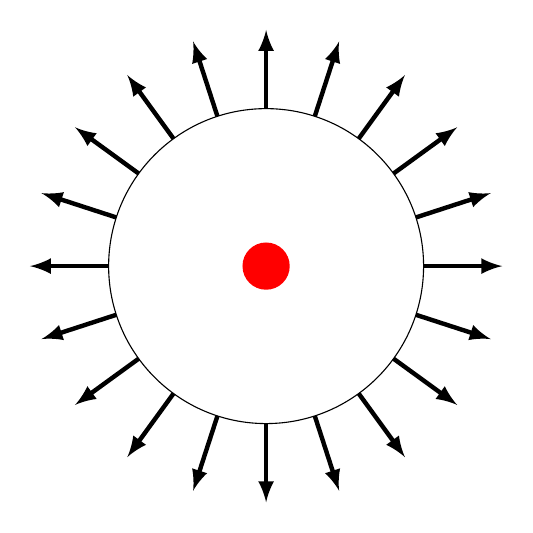
\begin{tikzpicture}
    \fill[red] (0,0) circle (3mm);
    \draw (0,0) circle (2cm);
    \foreach \x in {1,...,20}{\draw[ultra thick,-latex] ({\x*360/20}:2cm) -- ++({\x*360/20}:1cm);}
\end{tikzpicture}
\todo{Add robot figure here}

Two mazes are used (see Figure) similar to the ones in \cite{novelty_alone}.

\begin{figure}[H]
    \captionsetup[subfigure]{justification=centering}
    \centering
    \begin{mdframed}
        \begin{subfigure}[b]{0.45\textwidth}
            \centering
            \hspace*{2em}\scalebox{0.3}{%% Creator: Matplotlib, PGF backend
%%
%% To include the figure in your LaTeX document, write
%%   \input{<filename>.pgf}
%%
%% Make sure the required packages are loaded in your preamble
%%   \usepackage{pgf}
%%
%% and, on pdftex
%%   \usepackage[utf8]{inputenc}\DeclareUnicodeCharacter{2212}{-}
%%
%% or, on luatex and xetex
%%   \usepackage{unicode-math}
%%
%% Figures using additional raster images can only be included by \input if
%% they are in the same directory as the main LaTeX file. For loading figures
%% from other directories you can use the `import` package
%%   \usepackage{import}
%%
%% and then include the figures with
%%   \import{<path to file>}{<filename>.pgf}
%%
%% Matplotlib used the following preamble
%%
\begingroup%
\makeatletter%
\begin{pgfpicture}%
\pgfpathrectangle{\pgfpointorigin}{\pgfqpoint{6.400000in}{3.280000in}}%
\pgfusepath{use as bounding box, clip}%
\begin{pgfscope}%
\pgfsetbuttcap%
\pgfsetmiterjoin%
\definecolor{currentfill}{rgb}{1.000000,1.000000,1.000000}%
\pgfsetfillcolor{currentfill}%
\pgfsetlinewidth{0.000000pt}%
\definecolor{currentstroke}{rgb}{1.000000,1.000000,1.000000}%
\pgfsetstrokecolor{currentstroke}%
\pgfsetdash{}{0pt}%
\pgfpathmoveto{\pgfqpoint{0.000000in}{0.000000in}}%
\pgfpathlineto{\pgfqpoint{6.400000in}{0.000000in}}%
\pgfpathlineto{\pgfqpoint{6.400000in}{3.280000in}}%
\pgfpathlineto{\pgfqpoint{0.000000in}{3.280000in}}%
\pgfpathclose%
\pgfusepath{fill}%
\end{pgfscope}%
\begin{pgfscope}%
\pgfpathrectangle{\pgfqpoint{0.100000in}{0.100000in}}{\pgfqpoint{6.200000in}{3.080000in}}%
\pgfusepath{clip}%
\pgfsetbuttcap%
\pgfsetmiterjoin%
\definecolor{currentfill}{rgb}{0.600000,1.000000,0.600000}%
\pgfsetfillcolor{currentfill}%
\pgfsetlinewidth{1.003750pt}%
\definecolor{currentstroke}{rgb}{1.000000,1.000000,1.000000}%
\pgfsetstrokecolor{currentstroke}%
\pgfsetdash{}{0pt}%
\pgfpathmoveto{\pgfqpoint{0.565000in}{0.323300in}}%
\pgfpathcurveto{\pgfqpoint{0.595830in}{0.323300in}}{\pgfqpoint{0.625401in}{0.335470in}}{\pgfqpoint{0.647201in}{0.357129in}}%
\pgfpathcurveto{\pgfqpoint{0.669001in}{0.378789in}}{\pgfqpoint{0.681250in}{0.408169in}}{\pgfqpoint{0.681250in}{0.438800in}}%
\pgfpathcurveto{\pgfqpoint{0.681250in}{0.469431in}}{\pgfqpoint{0.669001in}{0.498811in}}{\pgfqpoint{0.647201in}{0.520471in}}%
\pgfpathcurveto{\pgfqpoint{0.625401in}{0.542130in}}{\pgfqpoint{0.595830in}{0.554300in}}{\pgfqpoint{0.565000in}{0.554300in}}%
\pgfpathcurveto{\pgfqpoint{0.534170in}{0.554300in}}{\pgfqpoint{0.504599in}{0.542130in}}{\pgfqpoint{0.482799in}{0.520471in}}%
\pgfpathcurveto{\pgfqpoint{0.460999in}{0.498811in}}{\pgfqpoint{0.448750in}{0.469431in}}{\pgfqpoint{0.448750in}{0.438800in}}%
\pgfpathcurveto{\pgfqpoint{0.448750in}{0.408169in}}{\pgfqpoint{0.460999in}{0.378789in}}{\pgfqpoint{0.482799in}{0.357129in}}%
\pgfpathcurveto{\pgfqpoint{0.504599in}{0.335470in}}{\pgfqpoint{0.534170in}{0.323300in}}{\pgfqpoint{0.565000in}{0.323300in}}%
\pgfpathclose%
\pgfusepath{stroke,fill}%
\end{pgfscope}%
\begin{pgfscope}%
\pgfpathrectangle{\pgfqpoint{0.100000in}{0.100000in}}{\pgfqpoint{6.200000in}{3.080000in}}%
\pgfusepath{clip}%
\pgfsetbuttcap%
\pgfsetmiterjoin%
\definecolor{currentfill}{rgb}{1.000000,0.200000,0.000000}%
\pgfsetfillcolor{currentfill}%
\pgfsetlinewidth{1.003750pt}%
\definecolor{currentstroke}{rgb}{1.000000,1.000000,1.000000}%
\pgfsetstrokecolor{currentstroke}%
\pgfsetdash{}{0pt}%
\pgfpathmoveto{\pgfqpoint{4.285000in}{1.524500in}}%
\pgfpathcurveto{\pgfqpoint{4.315830in}{1.524500in}}{\pgfqpoint{4.345401in}{1.536670in}}{\pgfqpoint{4.367201in}{1.558329in}}%
\pgfpathcurveto{\pgfqpoint{4.389001in}{1.579989in}}{\pgfqpoint{4.401250in}{1.609369in}}{\pgfqpoint{4.401250in}{1.640000in}}%
\pgfpathcurveto{\pgfqpoint{4.401250in}{1.670631in}}{\pgfqpoint{4.389001in}{1.700011in}}{\pgfqpoint{4.367201in}{1.721671in}}%
\pgfpathcurveto{\pgfqpoint{4.345401in}{1.743330in}}{\pgfqpoint{4.315830in}{1.755500in}}{\pgfqpoint{4.285000in}{1.755500in}}%
\pgfpathcurveto{\pgfqpoint{4.254170in}{1.755500in}}{\pgfqpoint{4.224599in}{1.743330in}}{\pgfqpoint{4.202799in}{1.721671in}}%
\pgfpathcurveto{\pgfqpoint{4.180999in}{1.700011in}}{\pgfqpoint{4.168750in}{1.670631in}}{\pgfqpoint{4.168750in}{1.640000in}}%
\pgfpathcurveto{\pgfqpoint{4.168750in}{1.609369in}}{\pgfqpoint{4.180999in}{1.579989in}}{\pgfqpoint{4.202799in}{1.558329in}}%
\pgfpathcurveto{\pgfqpoint{4.224599in}{1.536670in}}{\pgfqpoint{4.254170in}{1.524500in}}{\pgfqpoint{4.285000in}{1.524500in}}%
\pgfpathclose%
\pgfusepath{stroke,fill}%
\end{pgfscope}%
\begin{pgfscope}%
\pgfpathrectangle{\pgfqpoint{0.100000in}{0.100000in}}{\pgfqpoint{6.200000in}{3.080000in}}%
\pgfusepath{clip}%
\pgfsetrectcap%
\pgfsetroundjoin%
\pgfsetlinewidth{1.505625pt}%
\definecolor{currentstroke}{rgb}{0.121569,0.466667,0.705882}%
\pgfsetstrokecolor{currentstroke}%
\pgfsetdash{}{0pt}%
\pgfpathmoveto{\pgfqpoint{0.177500in}{0.177000in}}%
\pgfpathlineto{\pgfqpoint{4.672500in}{0.177000in}}%
\pgfusepath{stroke}%
\end{pgfscope}%
\begin{pgfscope}%
\pgfpathrectangle{\pgfqpoint{0.100000in}{0.100000in}}{\pgfqpoint{6.200000in}{3.080000in}}%
\pgfusepath{clip}%
\pgfsetrectcap%
\pgfsetroundjoin%
\pgfsetlinewidth{1.505625pt}%
\definecolor{currentstroke}{rgb}{0.121569,0.466667,0.705882}%
\pgfsetstrokecolor{currentstroke}%
\pgfsetdash{}{0pt}%
\pgfpathmoveto{\pgfqpoint{4.672500in}{0.177000in}}%
\pgfpathlineto{\pgfqpoint{4.672500in}{2.179000in}}%
\pgfusepath{stroke}%
\end{pgfscope}%
\begin{pgfscope}%
\pgfpathrectangle{\pgfqpoint{0.100000in}{0.100000in}}{\pgfqpoint{6.200000in}{3.080000in}}%
\pgfusepath{clip}%
\pgfsetrectcap%
\pgfsetroundjoin%
\pgfsetlinewidth{1.505625pt}%
\definecolor{currentstroke}{rgb}{0.121569,0.466667,0.705882}%
\pgfsetstrokecolor{currentstroke}%
\pgfsetdash{}{0pt}%
\pgfpathmoveto{\pgfqpoint{4.672500in}{2.179000in}}%
\pgfpathlineto{\pgfqpoint{0.177500in}{2.179000in}}%
\pgfusepath{stroke}%
\end{pgfscope}%
\begin{pgfscope}%
\pgfpathrectangle{\pgfqpoint{0.100000in}{0.100000in}}{\pgfqpoint{6.200000in}{3.080000in}}%
\pgfusepath{clip}%
\pgfsetrectcap%
\pgfsetroundjoin%
\pgfsetlinewidth{1.505625pt}%
\definecolor{currentstroke}{rgb}{0.121569,0.466667,0.705882}%
\pgfsetstrokecolor{currentstroke}%
\pgfsetdash{}{0pt}%
\pgfpathmoveto{\pgfqpoint{0.177500in}{2.179000in}}%
\pgfpathlineto{\pgfqpoint{0.177500in}{0.177000in}}%
\pgfusepath{stroke}%
\end{pgfscope}%
\begin{pgfscope}%
\pgfpathrectangle{\pgfqpoint{0.100000in}{0.100000in}}{\pgfqpoint{6.200000in}{3.080000in}}%
\pgfusepath{clip}%
\pgfsetrectcap%
\pgfsetroundjoin%
\pgfsetlinewidth{1.505625pt}%
\definecolor{currentstroke}{rgb}{0.121569,0.466667,0.705882}%
\pgfsetstrokecolor{currentstroke}%
\pgfsetdash{}{0pt}%
\pgfpathmoveto{\pgfqpoint{3.835500in}{2.179000in}}%
\pgfpathlineto{\pgfqpoint{0.999000in}{1.101000in}}%
\pgfusepath{stroke}%
\end{pgfscope}%
\begin{pgfscope}%
\pgfpathrectangle{\pgfqpoint{0.100000in}{0.100000in}}{\pgfqpoint{6.200000in}{3.080000in}}%
\pgfusepath{clip}%
\pgfsetrectcap%
\pgfsetroundjoin%
\pgfsetlinewidth{1.505625pt}%
\definecolor{currentstroke}{rgb}{0.121569,0.466667,0.705882}%
\pgfsetstrokecolor{currentstroke}%
\pgfsetdash{}{0pt}%
\pgfpathmoveto{\pgfqpoint{1.867000in}{0.177000in}}%
\pgfpathlineto{\pgfqpoint{1.231500in}{0.746800in}}%
\pgfusepath{stroke}%
\end{pgfscope}%
\begin{pgfscope}%
\pgfpathrectangle{\pgfqpoint{0.100000in}{0.100000in}}{\pgfqpoint{6.200000in}{3.080000in}}%
\pgfusepath{clip}%
\pgfsetrectcap%
\pgfsetroundjoin%
\pgfsetlinewidth{1.505625pt}%
\definecolor{currentstroke}{rgb}{0.121569,0.466667,0.705882}%
\pgfsetstrokecolor{currentstroke}%
\pgfsetdash{}{0pt}%
\pgfpathmoveto{\pgfqpoint{2.115000in}{1.501400in}}%
\pgfpathlineto{\pgfqpoint{1.758500in}{0.808400in}}%
\pgfusepath{stroke}%
\end{pgfscope}%
\begin{pgfscope}%
\pgfpathrectangle{\pgfqpoint{0.100000in}{0.100000in}}{\pgfqpoint{6.200000in}{3.080000in}}%
\pgfusepath{clip}%
\pgfsetrectcap%
\pgfsetroundjoin%
\pgfsetlinewidth{1.505625pt}%
\definecolor{currentstroke}{rgb}{0.121569,0.466667,0.705882}%
\pgfsetstrokecolor{currentstroke}%
\pgfsetdash{}{0pt}%
\pgfpathmoveto{\pgfqpoint{3.138000in}{0.177000in}}%
\pgfpathlineto{\pgfqpoint{2.254500in}{0.885400in}}%
\pgfusepath{stroke}%
\end{pgfscope}%
\begin{pgfscope}%
\pgfpathrectangle{\pgfqpoint{0.100000in}{0.100000in}}{\pgfqpoint{6.200000in}{3.080000in}}%
\pgfusepath{clip}%
\pgfsetrectcap%
\pgfsetroundjoin%
\pgfsetlinewidth{1.505625pt}%
\definecolor{currentstroke}{rgb}{0.121569,0.466667,0.705882}%
\pgfsetstrokecolor{currentstroke}%
\pgfsetdash{}{0pt}%
\pgfpathmoveto{\pgfqpoint{3.494500in}{2.025000in}}%
\pgfpathlineto{\pgfqpoint{2.921000in}{1.070200in}}%
\pgfusepath{stroke}%
\end{pgfscope}%
\begin{pgfscope}%
\pgfpathrectangle{\pgfqpoint{0.100000in}{0.100000in}}{\pgfqpoint{6.200000in}{3.080000in}}%
\pgfusepath{clip}%
\pgfsetrectcap%
\pgfsetroundjoin%
\pgfsetlinewidth{1.505625pt}%
\definecolor{currentstroke}{rgb}{0.121569,0.466667,0.705882}%
\pgfsetstrokecolor{currentstroke}%
\pgfsetdash{}{0pt}%
\pgfpathmoveto{\pgfqpoint{4.238500in}{0.177000in}}%
\pgfpathlineto{\pgfqpoint{3.417000in}{1.070200in}}%
\pgfusepath{stroke}%
\end{pgfscope}%
\begin{pgfscope}%
\pgfpathrectangle{\pgfqpoint{0.100000in}{0.100000in}}{\pgfqpoint{6.200000in}{3.080000in}}%
\pgfusepath{clip}%
\pgfsetrectcap%
\pgfsetroundjoin%
\pgfsetlinewidth{1.505625pt}%
\definecolor{currentstroke}{rgb}{0.121569,0.466667,0.705882}%
\pgfsetstrokecolor{currentstroke}%
\pgfsetdash{}{0pt}%
\pgfpathmoveto{\pgfqpoint{4.300500in}{2.179000in}}%
\pgfpathlineto{\pgfqpoint{3.773500in}{1.455200in}}%
\pgfusepath{stroke}%
\end{pgfscope}%
\end{pgfpicture}%
\makeatother%
\endgroup%
}
            \caption{Medium.}
        \end{subfigure}
        \begin{subfigure}[b]{0.5\textwidth}
            \centering
            \hspace*{5em}\scalebox{0.3}{%% Creator: Matplotlib, PGF backend
%%
%% To include the figure in your LaTeX document, write
%%   \input{<filename>.pgf}
%%
%% Make sure the required packages are loaded in your preamble
%%   \usepackage{pgf}
%%
%% and, on pdftex
%%   \usepackage[utf8]{inputenc}\DeclareUnicodeCharacter{2212}{-}
%%
%% or, on luatex and xetex
%%   \usepackage{unicode-math}
%%
%% Figures using additional raster images can only be included by \input if
%% they are in the same directory as the main LaTeX file. For loading figures
%% from other directories you can use the `import` package
%%   \usepackage{import}
%%
%% and then include the figures with
%%   \import{<path to file>}{<filename>.pgf}
%%
%% Matplotlib used the following preamble
%%
\begingroup%
\makeatletter%
\begin{pgfpicture}%
\pgfpathrectangle{\pgfpointorigin}{\pgfqpoint{6.400000in}{3.280000in}}%
\pgfusepath{use as bounding box, clip}%
\begin{pgfscope}%
\pgfsetbuttcap%
\pgfsetmiterjoin%
\definecolor{currentfill}{rgb}{1.000000,1.000000,1.000000}%
\pgfsetfillcolor{currentfill}%
\pgfsetlinewidth{0.000000pt}%
\definecolor{currentstroke}{rgb}{1.000000,1.000000,1.000000}%
\pgfsetstrokecolor{currentstroke}%
\pgfsetdash{}{0pt}%
\pgfpathmoveto{\pgfqpoint{0.000000in}{0.000000in}}%
\pgfpathlineto{\pgfqpoint{6.400000in}{0.000000in}}%
\pgfpathlineto{\pgfqpoint{6.400000in}{3.280000in}}%
\pgfpathlineto{\pgfqpoint{0.000000in}{3.280000in}}%
\pgfpathclose%
\pgfusepath{fill}%
\end{pgfscope}%
\begin{pgfscope}%
\pgfpathrectangle{\pgfqpoint{0.100000in}{0.100000in}}{\pgfqpoint{6.200000in}{3.080000in}}%
\pgfusepath{clip}%
\pgfsetbuttcap%
\pgfsetmiterjoin%
\definecolor{currentfill}{rgb}{0.600000,1.000000,0.600000}%
\pgfsetfillcolor{currentfill}%
\pgfsetlinewidth{1.003750pt}%
\definecolor{currentstroke}{rgb}{1.000000,1.000000,1.000000}%
\pgfsetstrokecolor{currentstroke}%
\pgfsetdash{}{0pt}%
\pgfpathmoveto{\pgfqpoint{0.658000in}{2.818100in}}%
\pgfpathcurveto{\pgfqpoint{0.688830in}{2.818100in}}{\pgfqpoint{0.718401in}{2.830270in}}{\pgfqpoint{0.740201in}{2.851929in}}%
\pgfpathcurveto{\pgfqpoint{0.762001in}{2.873589in}}{\pgfqpoint{0.774250in}{2.902969in}}{\pgfqpoint{0.774250in}{2.933600in}}%
\pgfpathcurveto{\pgfqpoint{0.774250in}{2.964231in}}{\pgfqpoint{0.762001in}{2.993611in}}{\pgfqpoint{0.740201in}{3.015271in}}%
\pgfpathcurveto{\pgfqpoint{0.718401in}{3.036930in}}{\pgfqpoint{0.688830in}{3.049100in}}{\pgfqpoint{0.658000in}{3.049100in}}%
\pgfpathcurveto{\pgfqpoint{0.627170in}{3.049100in}}{\pgfqpoint{0.597599in}{3.036930in}}{\pgfqpoint{0.575799in}{3.015271in}}%
\pgfpathcurveto{\pgfqpoint{0.553999in}{2.993611in}}{\pgfqpoint{0.541750in}{2.964231in}}{\pgfqpoint{0.541750in}{2.933600in}}%
\pgfpathcurveto{\pgfqpoint{0.541750in}{2.902969in}}{\pgfqpoint{0.553999in}{2.873589in}}{\pgfqpoint{0.575799in}{2.851929in}}%
\pgfpathcurveto{\pgfqpoint{0.597599in}{2.830270in}}{\pgfqpoint{0.627170in}{2.818100in}}{\pgfqpoint{0.658000in}{2.818100in}}%
\pgfpathclose%
\pgfusepath{stroke,fill}%
\end{pgfscope}%
\begin{pgfscope}%
\pgfpathrectangle{\pgfqpoint{0.100000in}{0.100000in}}{\pgfqpoint{6.200000in}{3.080000in}}%
\pgfusepath{clip}%
\pgfsetbuttcap%
\pgfsetmiterjoin%
\definecolor{currentfill}{rgb}{1.000000,0.200000,0.000000}%
\pgfsetfillcolor{currentfill}%
\pgfsetlinewidth{1.003750pt}%
\definecolor{currentstroke}{rgb}{1.000000,1.000000,1.000000}%
\pgfsetstrokecolor{currentstroke}%
\pgfsetdash{}{0pt}%
\pgfpathmoveto{\pgfqpoint{0.580500in}{0.292500in}}%
\pgfpathcurveto{\pgfqpoint{0.611330in}{0.292500in}}{\pgfqpoint{0.640901in}{0.304670in}}{\pgfqpoint{0.662701in}{0.326329in}}%
\pgfpathcurveto{\pgfqpoint{0.684501in}{0.347989in}}{\pgfqpoint{0.696750in}{0.377369in}}{\pgfqpoint{0.696750in}{0.408000in}}%
\pgfpathcurveto{\pgfqpoint{0.696750in}{0.438631in}}{\pgfqpoint{0.684501in}{0.468011in}}{\pgfqpoint{0.662701in}{0.489671in}}%
\pgfpathcurveto{\pgfqpoint{0.640901in}{0.511330in}}{\pgfqpoint{0.611330in}{0.523500in}}{\pgfqpoint{0.580500in}{0.523500in}}%
\pgfpathcurveto{\pgfqpoint{0.549670in}{0.523500in}}{\pgfqpoint{0.520099in}{0.511330in}}{\pgfqpoint{0.498299in}{0.489671in}}%
\pgfpathcurveto{\pgfqpoint{0.476499in}{0.468011in}}{\pgfqpoint{0.464250in}{0.438631in}}{\pgfqpoint{0.464250in}{0.408000in}}%
\pgfpathcurveto{\pgfqpoint{0.464250in}{0.377369in}}{\pgfqpoint{0.476499in}{0.347989in}}{\pgfqpoint{0.498299in}{0.326329in}}%
\pgfpathcurveto{\pgfqpoint{0.520099in}{0.304670in}}{\pgfqpoint{0.549670in}{0.292500in}}{\pgfqpoint{0.580500in}{0.292500in}}%
\pgfpathclose%
\pgfusepath{stroke,fill}%
\end{pgfscope}%
\begin{pgfscope}%
\pgfpathrectangle{\pgfqpoint{0.100000in}{0.100000in}}{\pgfqpoint{6.200000in}{3.080000in}}%
\pgfusepath{clip}%
\pgfsetrectcap%
\pgfsetroundjoin%
\pgfsetlinewidth{1.505625pt}%
\definecolor{currentstroke}{rgb}{0.121569,0.466667,0.705882}%
\pgfsetstrokecolor{currentstroke}%
\pgfsetdash{}{0pt}%
\pgfpathmoveto{\pgfqpoint{0.177500in}{0.177000in}}%
\pgfpathlineto{\pgfqpoint{0.177500in}{3.180000in}}%
\pgfusepath{stroke}%
\end{pgfscope}%
\begin{pgfscope}%
\pgfpathrectangle{\pgfqpoint{0.100000in}{0.100000in}}{\pgfqpoint{6.200000in}{3.080000in}}%
\pgfusepath{clip}%
\pgfsetrectcap%
\pgfsetroundjoin%
\pgfsetlinewidth{1.505625pt}%
\definecolor{currentstroke}{rgb}{0.121569,0.466667,0.705882}%
\pgfsetstrokecolor{currentstroke}%
\pgfsetdash{}{0pt}%
\pgfpathmoveto{\pgfqpoint{0.177500in}{3.180000in}}%
\pgfpathlineto{\pgfqpoint{3.200000in}{3.180000in}}%
\pgfusepath{stroke}%
\end{pgfscope}%
\begin{pgfscope}%
\pgfpathrectangle{\pgfqpoint{0.100000in}{0.100000in}}{\pgfqpoint{6.200000in}{3.080000in}}%
\pgfusepath{clip}%
\pgfsetrectcap%
\pgfsetroundjoin%
\pgfsetlinewidth{1.505625pt}%
\definecolor{currentstroke}{rgb}{0.121569,0.466667,0.705882}%
\pgfsetstrokecolor{currentstroke}%
\pgfsetdash{}{0pt}%
\pgfpathmoveto{\pgfqpoint{3.200000in}{3.180000in}}%
\pgfpathlineto{\pgfqpoint{3.200000in}{0.177000in}}%
\pgfusepath{stroke}%
\end{pgfscope}%
\begin{pgfscope}%
\pgfpathrectangle{\pgfqpoint{0.100000in}{0.100000in}}{\pgfqpoint{6.200000in}{3.080000in}}%
\pgfusepath{clip}%
\pgfsetrectcap%
\pgfsetroundjoin%
\pgfsetlinewidth{1.505625pt}%
\definecolor{currentstroke}{rgb}{0.121569,0.466667,0.705882}%
\pgfsetstrokecolor{currentstroke}%
\pgfsetdash{}{0pt}%
\pgfpathmoveto{\pgfqpoint{3.200000in}{0.177000in}}%
\pgfpathlineto{\pgfqpoint{0.177500in}{0.177000in}}%
\pgfusepath{stroke}%
\end{pgfscope}%
\begin{pgfscope}%
\pgfpathrectangle{\pgfqpoint{0.100000in}{0.100000in}}{\pgfqpoint{6.200000in}{3.080000in}}%
\pgfusepath{clip}%
\pgfsetrectcap%
\pgfsetroundjoin%
\pgfsetlinewidth{1.505625pt}%
\definecolor{currentstroke}{rgb}{0.121569,0.466667,0.705882}%
\pgfsetstrokecolor{currentstroke}%
\pgfsetdash{}{0pt}%
\pgfpathmoveto{\pgfqpoint{0.177500in}{0.854600in}}%
\pgfpathlineto{\pgfqpoint{0.983500in}{0.916200in}}%
\pgfusepath{stroke}%
\end{pgfscope}%
\begin{pgfscope}%
\pgfpathrectangle{\pgfqpoint{0.100000in}{0.100000in}}{\pgfqpoint{6.200000in}{3.080000in}}%
\pgfusepath{clip}%
\pgfsetrectcap%
\pgfsetroundjoin%
\pgfsetlinewidth{1.505625pt}%
\definecolor{currentstroke}{rgb}{0.121569,0.466667,0.705882}%
\pgfsetstrokecolor{currentstroke}%
\pgfsetdash{}{0pt}%
\pgfpathmoveto{\pgfqpoint{0.968000in}{0.931600in}}%
\pgfpathlineto{\pgfqpoint{0.968000in}{2.517800in}}%
\pgfusepath{stroke}%
\end{pgfscope}%
\begin{pgfscope}%
\pgfpathrectangle{\pgfqpoint{0.100000in}{0.100000in}}{\pgfqpoint{6.200000in}{3.080000in}}%
\pgfusepath{clip}%
\pgfsetrectcap%
\pgfsetroundjoin%
\pgfsetlinewidth{1.505625pt}%
\definecolor{currentstroke}{rgb}{0.121569,0.466667,0.705882}%
\pgfsetstrokecolor{currentstroke}%
\pgfsetdash{}{0pt}%
\pgfpathmoveto{\pgfqpoint{0.983500in}{1.732400in}}%
\pgfpathlineto{\pgfqpoint{2.549000in}{2.594800in}}%
\pgfusepath{stroke}%
\end{pgfscope}%
\begin{pgfscope}%
\pgfpathrectangle{\pgfqpoint{0.100000in}{0.100000in}}{\pgfqpoint{6.200000in}{3.080000in}}%
\pgfusepath{clip}%
\pgfsetrectcap%
\pgfsetroundjoin%
\pgfsetlinewidth{1.505625pt}%
\definecolor{currentstroke}{rgb}{0.121569,0.466667,0.705882}%
\pgfsetstrokecolor{currentstroke}%
\pgfsetdash{}{0pt}%
\pgfpathmoveto{\pgfqpoint{1.293500in}{3.180000in}}%
\pgfpathlineto{\pgfqpoint{1.774000in}{2.625600in}}%
\pgfusepath{stroke}%
\end{pgfscope}%
\begin{pgfscope}%
\pgfpathrectangle{\pgfqpoint{0.100000in}{0.100000in}}{\pgfqpoint{6.200000in}{3.080000in}}%
\pgfusepath{clip}%
\pgfsetrectcap%
\pgfsetroundjoin%
\pgfsetlinewidth{1.505625pt}%
\definecolor{currentstroke}{rgb}{0.121569,0.466667,0.705882}%
\pgfsetstrokecolor{currentstroke}%
\pgfsetdash{}{0pt}%
\pgfpathmoveto{\pgfqpoint{0.177500in}{1.332000in}}%
\pgfpathlineto{\pgfqpoint{0.611500in}{1.963400in}}%
\pgfusepath{stroke}%
\end{pgfscope}%
\begin{pgfscope}%
\pgfpathrectangle{\pgfqpoint{0.100000in}{0.100000in}}{\pgfqpoint{6.200000in}{3.080000in}}%
\pgfusepath{clip}%
\pgfsetrectcap%
\pgfsetroundjoin%
\pgfsetlinewidth{1.505625pt}%
\definecolor{currentstroke}{rgb}{0.121569,0.466667,0.705882}%
\pgfsetstrokecolor{currentstroke}%
\pgfsetdash{}{0pt}%
\pgfpathmoveto{\pgfqpoint{3.200000in}{2.348400in}}%
\pgfpathlineto{\pgfqpoint{1.448500in}{1.501400in}}%
\pgfusepath{stroke}%
\end{pgfscope}%
\begin{pgfscope}%
\pgfpathrectangle{\pgfqpoint{0.100000in}{0.100000in}}{\pgfqpoint{6.200000in}{3.080000in}}%
\pgfusepath{clip}%
\pgfsetrectcap%
\pgfsetroundjoin%
\pgfsetlinewidth{1.505625pt}%
\definecolor{currentstroke}{rgb}{0.121569,0.466667,0.705882}%
\pgfsetstrokecolor{currentstroke}%
\pgfsetdash{}{0pt}%
\pgfpathmoveto{\pgfqpoint{0.968000in}{0.947000in}}%
\pgfpathlineto{\pgfqpoint{2.161500in}{0.562000in}}%
\pgfusepath{stroke}%
\end{pgfscope}%
\end{pgfpicture}%
\makeatother%
\endgroup%
}
            \caption{Hard.}
        \end{subfigure}
    \end{mdframed}
    \caption{The robot must navigate from the green point to the red in order to solve the maze.
             (b) is more deceptive than (a).}
    \label{mazes}
\end{figure}

\subsection{Novelty search variants studied}
Describe the different variants that will be compared.

\subsection{Experimental design}
Describe how the experiments will be run. What statistics will be collected and why.
test